% System architecture.

\section{System architecture}\label{sec:architecture}

DinHot is an instance of a product archetype in which the science runs offline, its results are committed, and a static web workbench replays them and re-runs what is light enough, live. Figure~\ref{fig:dataflow} shows the data flow: the case records enter through the first contract, the named stages compute and score every method, the gates check the result, the second contract writes the artifacts, and three lanes serve them. The base (the layout, the contracts, the stage names, the lanes and the guards) is carried by the product template and its shared shell; the core is DinHot's own: the engine, the methods, the cases and the views.

\begin{figure}[t]
\centering
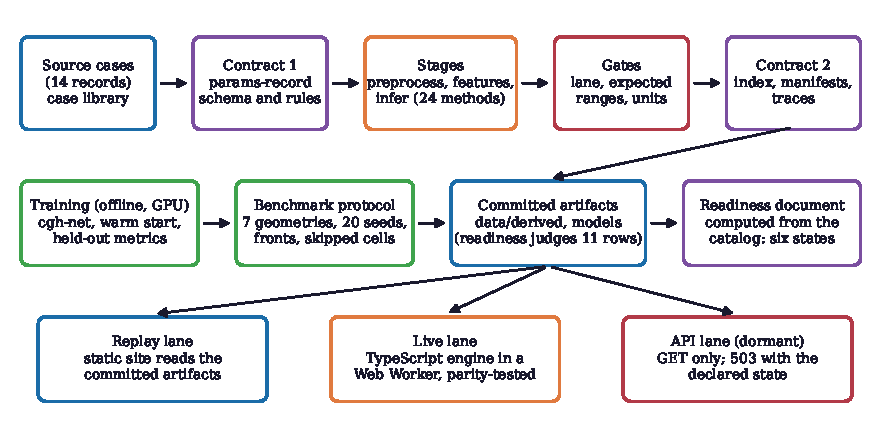
\includegraphics[width=\textwidth]{fig-dataflow.pdf}
\caption{Data flow of the build: the case records pass the first contract, the stages run every valid method with the same seed and score it, the gates check lane, expected ranges and units, and the second contract writes the artifacts that the replay, live and dormant API lanes serve; training and the benchmark are offline and write committed artifacts too.}
\label{fig:dataflow}
\end{figure}

\subsection{The staged pipeline}\label{sec:arch-stages}

The pipeline orchestrates named stages whose names and signatures are frozen by the base, and whose bodies are DinHot's. Every stage is deterministic, typed, seeded and independently testable. Table~\ref{tab:stages} lists them with their inputs, outputs and artifacts. The per-case bake runs, in order: the contract-1 record, the methods through the registry, the expected ranges, the lane measurement, the maps and drivers, the trace within the byte gate, the units gate and the manifest. It never raises for a method or a gate problem, so that one bad case does not hide the others: the failures are collected and one error names case, method or driver and metric at the end. The cases bake in parallel, one case per process, at most twelve processes with one linear-algebra thread each. The canonical bake is an explicit release operation and never runs in continuous integration; tests and quick runs write to a sandbox so that they cannot change the committed evidence.

\begin{table}[t]
\centering\footnotesize
\caption{The stages of the pipeline: the work each does, what it reads and what it writes; the training and evaluation stages run locally on a graphics processor and never in continuous integration or in the browser.}
\label{tab:stages}
\begin{tabular}{@{}l >{\raggedright\arraybackslash}p{0.31\textwidth} >{\raggedright\arraybackslash}p{0.23\textwidth} >{\raggedright\arraybackslash}p{0.23\textwidth}@{}}
\toprule
Stage & Work & Reads & Writes\\
\midrule
preprocess & contract 1: schema and the rules a schema cannot state; a rejected record carries its reason & case source document & accepted records\\
feature extraction & derived geometry: trap count, extent, smallest spacing in bins, fraction of the half field used & accepted records & per-record features\\
train & offline training of the two learned models & generated training sets & model card, graph, training record\\
infer & every valid method through the registry with the same seed and budget; independent scoring; camera, particle and rearrangement drivers & records, registry & per-method results\\
evaluate & held-out metrics of the model slots & held-out sets, graphs & model metrics, evidence\\
export & contract 2: the compact trace and the manifest with the lane and gate outcomes & results, drivers & traces, manifests, index\\
benchmark & the benchmark protocol over the registry & registry, geometries & benchmark results\\
\bottomrule
\end{tabular}
\end{table}

\subsection{The engine and the method interface}\label{sec:arch-engine}

The engine lives in a folder of the pipeline package and is documented card by card in the frameworks of the repository; it is not a package of its own. A method is a module with a specification and a run function; the registry discovers it, and the same interface serves the bake, the benchmark and the TypeScript port. The specification names the method's identifier, family, lane (live, both or baked), supported target kinds and dimensions. The run function takes the optical setup, the target, an optional device, a budget, the random generator and an optional starting phase, plus the keyword parameters of Table~\ref{tab:defaults}, and returns a result with the phase, a history with one entry per iteration (iteration, efficiency, uniformity, relative standard deviation and time), the fields at the traps and a metadata record. Of the \nLadder{} methods, \nLiveMethods{} are live or both and \nBakedMethods{} are baked. A method that does not accept a target refuses it with an error that names the supported kind, so a missing combination is a declared state and not a silent fall-back.

\begin{table}[t]\centering\scriptsize\setlength{\tabcolsep}{4pt}
\caption{Keyword defaults of every method, read from the signature of its \texttt{run} function by \texttt{params.py}, in two blocks; a default of \texttt{unset} is chosen at run time from the target, as the method section states, and methods with no keyword take only the interface arguments.}\label{tab:defaults}
\begin{tabular}{@{}>{\raggedright\arraybackslash}p{0.17\textwidth} l l @{\hskip 1.2em} >{\raggedright\arraybackslash}p{0.17\textwidth} l l@{}}\toprule Method & Keyword & Default & Method & Keyword & Default\\\midrule
device-aware weighted GS & \texttt{steps} & 3 & direct search & \texttt{f} & 0.5\\
 & \texttt{warm} & 12 &  & \texttt{levels} & 8\\
 & \texttt{weights} & true &  & \texttt{max\_trials} & unset\\
flicker-bounded phase-continuous sequence & \texttt{destination} & unset & conjugate-gradient minimization & \texttt{t} & unset\\
 & \texttt{frames} & 13 &  & \texttt{efficiency} & unset\\
 & \texttt{frame\_iterations} & 10 & Wirtinger gradient descent with Adam & \texttt{lr} & 1\\
 & \texttt{end\_phases} & unset &  & \texttt{efficiency} & unset\\
 & \texttt{phase\_velocity\_max} & 0.3 & closed-loop weighted GS & \texttt{variant} & nogrette\\
 & \texttt{n\_fix} & 12 &  & \texttt{gain} & 0.7\\
learned warm start & \texttt{n\_fix} & 12 &  & \texttt{camera} & unset\\
 & \texttt{form} & point &  & \texttt{n\_inner} & unset\\
 & \texttt{models\_dir} & unset &  & \texttt{n\_start} & 30\\
aberration-robust hologram & \texttt{q} & 8 &  & \texttt{start} & gsw\\
 & \texttt{lr} & 0.02 & device-aware CG with pixel crosstalk & \texttt{t} & unset\\
 & \texttt{warm} & 30 &  & \texttt{efficiency} & unset\\
 & \texttt{aberration} & 0.02 & Zernike correction & \texttt{mode} & recover\\
 & \texttt{pointing\_bins} & 0 &  & \texttt{injected} & unset\\
 & \texttt{design} & unset &  & \texttt{known} & unset\\
 & \texttt{level\_fraction} & 0.9 &  & \texttt{camera} & unset\\
efficiency-uniformity Pareto front & \texttt{n\_lambda} & 20 &  & \texttt{modes} & 4 to 11\\
 & \texttt{warm} & 30 &  & \texttt{trial\_waves} & 0.06\\
superposition of prisms and lenses & (none) &  &  & \texttt{base\_iterations} & 30\\
random superposition & (none) &  & Laguerre-Gaussian vortex traps & \texttt{charge} & unset\\
random mask & (none) &  & Hungarian assignment with phase interpolation & \texttt{atoms} & unset\\
GS & \texttt{form} & unset &  & \texttt{alpha} & 1.5\\
 & \texttt{start\_waves} & 20 &  & \texttt{max\_step\_bins} & unset\\
generalized adaptive additive GS & \texttt{alpha} & 0.5 &  & \texttt{n\_fix} & 12\\
 & \texttt{form} & auto & multi-plane CNN hologram & \texttt{models\_dir} & unset\\
 & \texttt{scale} & mean &  & \texttt{refine} & true\\
weighted GS & \texttt{form} & auto & optimal-transport initialized MRAF & \texttt{mix} & 0.4\\
phase-fixed weighted GS & \texttt{n\_fix} & 12 &  & \texttt{eps} & 0.001\\
 & \texttt{form} & auto &  & \texttt{ot\_iterations} & 200\\
mixed-region amplitude freedom & \texttt{mixing} & 0.3 & volumetric 3D GS & \texttt{dz\_m} & unset\\
 & \texttt{start\_waves} & 20 &  & \texttt{nz} & unset\\
\bottomrule\end{tabular}\end{table}


A method reports its own history, but the score that the manifest and the benchmark carry is recomputed by the scorer from the final phase, through the same forward model for every method and through the case's device and aberration. A method therefore cannot grade itself, and the methods are compared on one footing. The forward model, the device model, the metrics, the trap physics, the particle dynamics, the emulated camera and the portable random generator are the physics components that every method works inside; the components are described by the equations of Section~\ref{sec:problem}.

\subsection{Determinism and the trace}\label{sec:arch-determinism}

A run is a pure function of its parameters and its seed. There is no global random generator anywhere: every random draw goes through a portable generator of the xoshiro128 family seeded by SplitMix32~\cite{blackman}, whose uniforms the TypeScript port reproduces bit for bit and whose normals it reproduces to rounding. The draw order is part of the contract and is fixed in each module's documentation (the starts, the camera gains and noise, the device flicker, the particle noise). Every method of a case is given the same seed, so all of them start from the same random numbers and the same budget. Same inputs give byte-identical artifacts: the manifest carries no clock, and the only measured quantity behind it, the run time that decides the lane, is stored as a lane label and the deterministic budgets.

The trace is decimated and not the raw state (Section~\ref{sec:data-trace}): histories to at most 200 points, the reference method's phase in 256 levels and its focal intensity in decibels with a floor, an axial cut for three-dimensional cases, trajectories to at most 4000 points and rearrangement to at most 120 frames. Training data sets and checkpoints stay in the data root and never in the repository; only the compact artifacts, the released models and their cards are committed and shipped.

\subsection{The gates}\label{sec:arch-gates}

Three pipeline gates stand between a method's output and a committed artifact, and a fourth, measured on the built site, belongs to the web. The lane gate decides, by measurement, whether a case may be re-run live in the browser. The unit of judgement is the case's reference method; the case is live when that method's lane is live or both, one run at the case's own grid and budget takes at most the run budget of \liveBudgetMs{} ms, and the trace is within \liveTraceKiB{} KiB. Every method of the case also gets a lane of its own, and a method labelled live that does not fit is baked, never silently live. The cost judged is one run after a warm-up as the median of three, because timing the whole case once, validation and cold start included, made the lane label depend on bake order.

The expected-range gate states, for every case, a numeric range for named metrics (the metrics of the reference method, the case metrics measured by a driver, and the metrics of each method), and the bake fails on a value outside it, naming the case, the method and the metric. An expectation written only as prose can be wrong for months without anyone noticing; the ranges are measured on three seeds, each range the wider of ten percent around the median and the seed spread, and a range stays provisional where no published band sets it. The units gate checks, in the bake and again over the shipped artifacts, that every observable is in its physical domain and in the units of the question it answers: efficiency, uniformity and the fractions between zero and one; the relative standard deviation in percent between zero and a thousand; trap intensities relative to the mean trap; positions in micrometres inside the unaliased field; times in seconds, stiffness in piconewtons per micrometre and frequencies in hertz. The relative standard deviation and the uniformity are recomputed from the per-trap intensities and must agree, so a fraction written where a percent belongs fails.

\subsection{The lanes and the live engine}\label{sec:live}

The offline lane bakes every case with every valid method, checks each against its expected ranges and runs the benchmark and the units gate; training runs locally only. The replay lane serves the committed artifacts, copied into the site and fetched with the version in the address; the copy script stops the build when the released graph is absent or its size or checksum is not the card's. The live lane is a TypeScript port of the forward models, the device model and the live methods, running in a Web Worker so that the interface never blocks, with the fast Fourier transform in double precision (the fft.js library). An optional WebGPU backend runs the Fourier-form iterations of plain GS, weighted GS and phase-fixed weighted GS for ideal-device point traps on bins with no depth offset and no vortex, and every absent, ineligible or failing GPU run takes the CPU path and records the reason; an agreement check inside every GPU run compares the trap fields with the CPU result.

At the live grid ($256^2$ padded to $512^2$) a weighted GS iteration took about \liveIterMs{} ms in Node 24, and in the browser's worker 30 iterations on C02 took \liveWorkerS{} s, inside the lane budget. On \liveAdapter{}, 30 iterations of phase-fixed weighted GS took \liveGpuS{} s with the GPU backend against \liveCpuS{} s on the CPU path in the same browser. The Python engine writes \liveFixtures{} reference documents and \liveTests{} parity tests compare the TypeScript engine with them, each quantity within the tolerance its document states (at most $\liveTol$ absolute). The live lane is held to the Python engine by tests over fixtures that the Python engine writes: the ported methods are exactly those whose Python lane is live or both, and every other id raises a not-live error and is replayed from the bake. The methods that are baked and replayed are labelled as such in the interface, and the workbench labels every map with its lane. The ONNX runtime for the web runs the released network of Section~\ref{sec:m17} on one thread, since the static host sends no cross-origin isolation headers.

\subsection{The API lane and the deployment}\label{sec:arch-api}

The API lane is dormant: a read-only layer over the committed documents that answers 503 with the declared state while nothing is baked or a route's document is absent. It exists so that the product keeps the same contracts if a server is added, and it is tested against its OpenAPI document. The site itself is static: every computation runs in the browser or was baked offline and is replayed, and the deployment is the upload of the built site to a static host after the main branch passes the guards. The measured gate walks the built site at five sizes, in both themes and both languages, and a person reads its captures; the gate measures and does not judge content. The browser measurements behind the live design (the timings above, the memory of the point-trap plan and the GPU buffers) are quoted from the product's record of measured resources, and each states who measured it and on what.
